\documentclass[../../main.tex]{subfiles}
\begin{document}

{\bf [解答]}

与えられた関数
\begin{align}
  \begin{cases}
    f(x) = x(x-a)(b-x) \\
    g(x) = px^2 - qx
  \end{cases}\label{eq:1}
\end{align}
および
\begin{align}
  0 < a < b <c \label{eq:2}
\end{align}
について考える．

新しく
\begin{align}
  h(x) = f(x) - g(x) \label{eq:3}
\end{align}
に対して$x \le c$で常に$h(x) \ge 0$となる$(p,q)$を探せば良い．

一階微分を計算すると
\begin{align}
  h'(x) = -3x^2 + 2(a+b-p)x - ab + q \label{eq:4}
\end{align}
である．

さて，$f(x)=0, g(x)=0$の解はそれぞれ $x = 0, a, b$ と $x = 0, \dfrac{q}{p}$ だからグラフは図のようにな
る．

% f(x)=0, g(x)=0
\begin{figure}[htb]
  \centering
  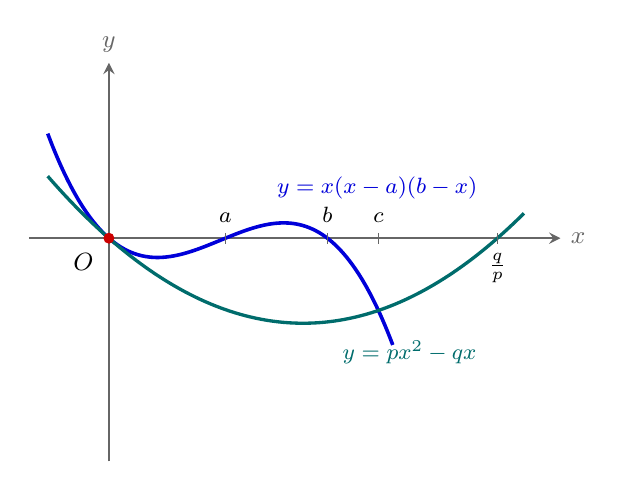
\begin{tikzpicture}[x=1.85cm, y=1.35cm, >=stealth,
    every node/.style={font=\small}]
    % Illustrative values: a=0.8, b=1.5, c=1.75, p=0.45, q=ab=1.2.
    % Then q/p = 8/3 ≈ 2.667, and f(x)-g(x) = x^2(1.85-x) >= 0 for x <= c.
    \draw[->, thick, gray!80!black] (-0.55,0) -- (3.1,0) node[right] {$x$};
    \draw[->, thick, gray!80!black] (0,-2.1) -- (0,1.65) node[above] {$y$};
    \draw[line width=1.3pt, blue!85!black, domain=-0.42:1.95,
    samples=100, smooth] plot (\x, {\x*(\x-0.8)*(1.5-\x)});
    \draw[line width=1.2pt, teal!85!black, domain=-0.42:2.85,
    samples=100, smooth] plot (\x, {0.45*\x*\x-1.2*\x});
    \node[circle, fill=red!80!black, inner sep=1.4pt] at (0,0) {};
    \node[below left=2pt] at (0,0) {$O$};
    \node[above right=2pt, blue!85!black, font=\footnotesize] at (1.05,0.22)
    {$y=x(x-a)(b-x)$};
    \node[below right=2pt, teal!85!black, font=\footnotesize] at (1.5,-0.82)
    {$y=px^2-qx$};
    \foreach \x/\name/\pos in {0.8/a/above, 1.5/b/above, 1.85/c/above, 2.6667/{\frac{q}{p}}/below} {
      \draw[gray!80!black] (\x,0.05) -- (\x,-0.05);
      \node[\pos=2pt, font=\footnotesize] at (\x,0) {$\name$};
    }
  \end{tikzpicture}
  \caption{原点で接する二つのグラフの一例（$0<a<b<c$）}
  \label{fig:1962_4_tangent_graphs}
\end{figure}

したがって，$h(x) \ge 0$となるためには$y=f(x), y=g(x)$が $x=0$ で接する（すなわち$h'(x)=0$である）ことが必要で，
\begin{align}
  h'(0)=0 \iff -q = -ab \iff q = ab \label{eq:5}
\end{align}
である．\cref{eq:4}に代入すると
\begin{align}
  h'(x) = x [ -3x + 2(a+b-p) ] \label{eq:6}
\end{align}
を得る．従って$a+b-p$の符号に応じて増減表は以下のようになる．

\begin{table}[htb]
  \centering
  \caption{$a+b-p$ の符号に応じた $h(x)$ の増減表}
  \label{tab:1962_4_hx_variation}
  \renewcommand{\arraystretch}{1.4}
  \begin{tabular}{c|ccccc}
    \multicolumn{6}{c}{$a+b-p > 0$ のとき} \\[2pt]
    \hline
    $x$ & $\dots$ & $0$ & $\dots$ & $\dfrac{2}{3}(a+b-p)$ & $\dots$ \\ \hline
    $h'(x)$ & $-$ & $0$ & $+$ & $0$ & $-$ \\ \hline
    $h(x)$ & $\searrow$ & $0$ & $\nearrow$ & 極大 & $\searrow$ \\ \hline
  \end{tabular}
  \hspace{1.2cm}
  \begin{tabular}{c|ccccc}
    \multicolumn{6}{c}{$a+b-p < 0$ のとき（$a+b-p=0$ も $x>0$ で単調減少）} \\[2pt]
    \hline
    $x$ & $\dots$ & $\dfrac{2}{3}(a+b-p)$ & $\dots$ & $0$ & $\dots$ \\ \hline
    $h'(x)$ & $-$ & $0$ & $+$ & $0$ & $-$ \\ \hline
    $h(x)$ & $\searrow$ & 極小 & $\nearrow$ & $0$ & $\searrow$ \\ \hline
  \end{tabular}
\end{table}

このうち，$x \le c$の範囲で$h'(x) \ge 0$となりうるのは
\begin{align}
  0 < a+b-p \label{eq:7}
\end{align}
の方である．さらに$c$の値に応じて場合分けする．

\subparagraph{$c < \dfrac{2}{3}(a+b)$ の時}

\begin{table}[htb]
  \centering
  \caption{$c \le \dfrac{2}{3}(a+b-p)$ となる $p$ をとったときの $h(x)$ の増減表（$x \le c$）}
  \label{tab:1962_4_case1}
  \renewcommand{\arraystretch}{1.4}
  \begin{tabular}{c|cccc|cc}
    \hline
    $x$ & $\dots$ & $0$ & $\dots$ & $c$ & $\dots$ & $\dfrac{2}{3}(a+b-p)$ \\ \hline
    $h'(x)$ & $-$ & $0$ & $+$ & & $+$ & $0$ \\ \hline
    $h(x)$ & $\searrow$ & $0$ & $\nearrow$ & $h(c)$ & $\nearrow$ & 極大 \\ \hline
  \end{tabular}
\end{table}

$c \le \dfrac{2}{3}(a+b-p)$ となるよう $p (>0)$ がとれて，この時 $h(x)$ は $x=0$ で $\min 0$ をとるから，題意を満たす $p, q$ が存在する．

\subparagraph{$c \ge \dfrac{2}{3}(a+b)$ の時}

\begin{table}[htb]
  \centering
  \caption{$\dfrac{2}{3}(a+b-p) < c$ のときの $h(x)$ の増減表（$x \le c$）}
  \label{tab:1962_4_case2}
  \renewcommand{\arraystretch}{1.4}
  \begin{tabular}{c|cccccc}
    \hline
    $x$ & $\dots$ & $0$ & $\dots$ & $\dfrac{2}{3}(a+b-p)$ & $\dots$ & $c$ \\ \hline
    $h'(x)$ & $-$ & $0$ & $+$ & $0$ & $-$ & \\ \hline
    $h(x)$ & $\searrow$ & $0$ & $\nearrow$ & 極大 & $\searrow$ & $h(c)$ \\ \hline
  \end{tabular}
\end{table}

この時は$\dfrac{2}{3}(a+b-p) < c$ となって，
$h(x)$ は，$x=0$ 又は $x=c$ で $\min$ をとる．$f(c)$を具体的に計算すると
\begin{align}
  f(c)
  &= -c(c-a)(c-b) - pc^2 + abc \\
  &= c [ -(c-a)(c-b) - pc + ab ] \\
  &= c^2 [ -c + (a+b-p) ]
\end{align}
だから，$c < a+b$ の時は，$f(c) \ge 0$ となる $p$ がとれて，題意を満たす $(p, q)$ が存在する．
逆に$c \ge a+b$ の時，$f(c) < 0$ となって条件は満たさず不適である．
以上から$c < a+b$の時は題意の$(p,q)$が存在する．
\casesend

以上から求める条件は，
\begin{align}
  \begin{cases}
    C < a+b \text{ の時，} (p, q) \text{ は存在する} \\
    C \ge a+b \text{ の時，存在しない}
  \end{cases}
\end{align}
である．

\newpage

\end{document}
